\documentclass[9pt, aspectratio=169]{beamer}
\usepackage{FiraSans}
\usetheme[subsectionpage=progressbar]{metropolis}
\usepackage[utf8]{inputenc}
\usepackage{amsmath}
\usepackage{amsfonts}
\usepackage{amssymb}
\usepackage{multicol}
\usepackage{tikz}
\usepackage{caption}
\usepackage{xcolor}
\usepackage[T1]{fontenc} 
\usepackage[skins]{tcolorbox}
\author{Nicola Roman\`o - nicola.romano@ed.ac.uk}
\title{Lecture 11 - Machine learning in image analysis - coding session} 
\setlength{\fboxsep}{0pt}
\setbeamertemplate {footline}{\begin{scriptsize}\hfill\insertframenumber ~of \inserttotalframenumber\kern1em\vskip5pt\end{scriptsize}}

% Remove "Figure" in front of captions
% See https://tex.stackexchange.com/questions/82456/how-to-remove-figure-caption-prefix-figure-in-beamer
\captionsetup{labelformat=empty,labelsep=none}

\titlegraphic{\centering 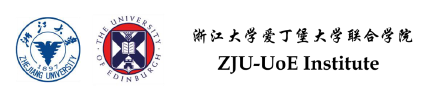
\includegraphics[scale=.5]{instituteLogo.png}}
\date{}

\begin{document}

\newtcolorbox{codebox}{enhanced,
    top=2pt,
    left=2pt,
    right=2pt,
    bottom=2pt,
    boxrule=0pt,
    leftrule=5pt,
    sharp corners,
    colback=gray!20,
    colframe=blue!60!black}

\begin{frame}
    \titlepage
\end{frame}

\begin{frame}
    {The general process}
    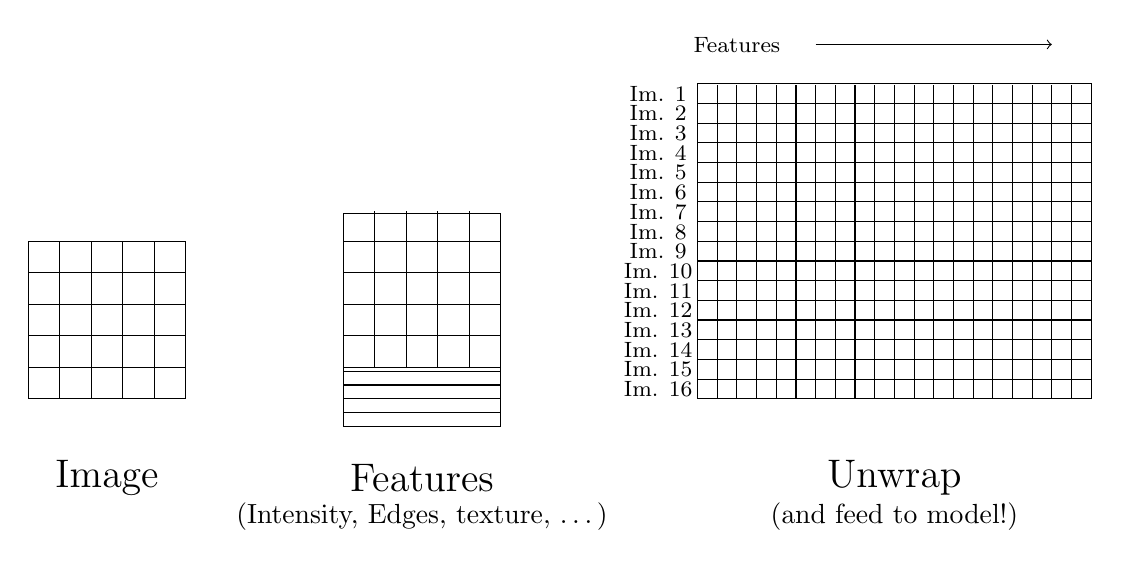
\begin{tikzpicture}
        \node at(1, -1) {\Large Image};
        \draw [fill=white] (0, 0) rectangle (2, 2);
        \draw [step=0.4] (0.01, 0.01) grid (1.99, 1.99);

        % Features
        \node at (5, -1) {\Large Features};
        \node at (5, -1.5) {\normalsize (Intensity, Edges, texture, \dots)};

        \foreach \y in {-10, -5, ..., 10}
        \draw [fill=white, yshift=\y] (4, 0) rectangle (6, 2);
        \draw [step=0.4] (4.01, 0.39) grid (5.99, 2.38);

        % Unwrap
        \draw (8.5, 0) rectangle (13.5, 4);
        \draw [step=0.25] (8.51, 0.01) grid (13.51, 3.99);

        \node at (11, -1) {\Large Unwrap};
        \node at (11, -1.5) {\normalsize (and feed to model!)};

        \foreach \i [count=\n] in {3.875, 3.625, ..., 0}
        \node at (8, \i) {\footnotesize Im. \n};
        \node at (9, 4.5) {\footnotesize Features};
        \draw [->] (10, 4.5) -- (13, 4.5);
    \end{tikzpicture}
\end{frame}

\begin{frame}
    {Supervised vs unsupervised ML}
    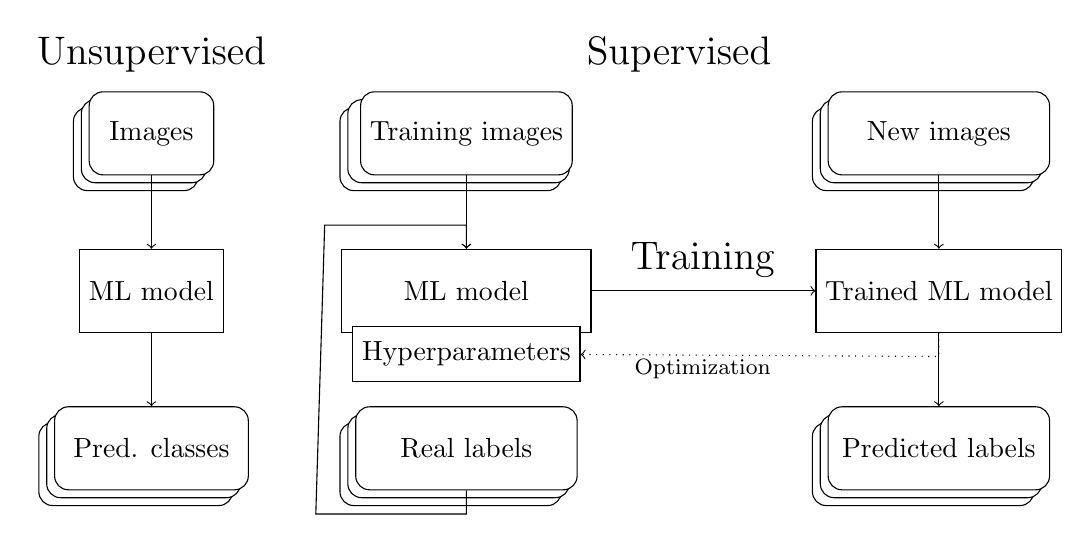
\begin{tikzpicture}
        \node at(0, 1) {\Large Unsupervised};

        \node[draw, rectangle, rounded corners=5pt, minimum height=3em, minimum width = 4.5em, fill=white] at (-0.2,-0.2) {};
        \node[draw, rectangle, rounded corners=5pt, minimum height=3em, minimum width = 4.5em, fill=white] at (-0.1,-0.1) {};
        \node[draw, rectangle, rounded corners=5pt, minimum height=3em, minimum width = 4.5em, fill=white] (img) at (0,0) {Images};
        \node[draw, rectangle, fill=white, minimum height=3em] (model2) at (0,-2) {ML model};

        \node[draw, rectangle, rounded corners=5pt, minimum height=3em, minimum width = 7em, fill=white] at (-0.2,-4.2) {};
        \node[draw, rectangle, rounded corners=5pt, minimum height=3em, minimum width = 7em, fill=white] at (-0.1,-4.1) {};
        \node[draw, rectangle, rounded corners=5pt, minimum height=3em, minimum width = 7em, fill=white] (classes) at (0,-4) {Pred. classes};

        \draw [->] (img) -- (model2);
        \draw [->] (model2) -- (classes);
        
        \node at(6.7, 1) {\Large Supervised};

        \node[draw, rectangle, rounded corners=5pt, minimum height=3em, minimum width = 8em, fill=white] at (3.8,-0.2) {};
        \node[draw, rectangle, rounded corners=5pt, minimum height=3em, minimum width = 8em, fill=white] at (3.9,-.1) {};
        \node[draw, rectangle, rounded corners=5pt, minimum height=3em, fill=white] (train) at (4,0) {Training images};

        \node[draw, rectangle, rounded corners=5pt, minimum height=3em, minimum width = 8em, fill=white] at (3.8,-4.2) {};
        \node[draw, rectangle, rounded corners=5pt, minimum height=3em, minimum width = 8em, fill=white] at (3.9,-4.1) {};
        \node[draw, rectangle, rounded corners=5pt, minimum height=3em, minimum width = 8em, fill=white] (labels) at (4,-4) {Real labels};

        \node[draw, rectangle, fill=white, minimum height=3em, minimum width = 9em] (model) at (4,-2) {ML model};
        \node[draw, rectangle, fill=white, minimum height=2em] (hyperparam) at (4,-2.8) {Hyperparameters};

        \node at (7, -1.6) {\Large Training};
        \node[draw, rectangle, fill=white, minimum height=3em] (modeltrained) at (10,-2) {Trained ML model};

        \draw [->] (train) -- (model);
        \draw [->] (labels) |-([shift={(-5mm,-3mm)}]labels.south west)-- ([shift={(-18mm,3mm)}]model.north)-| (model);
        \draw [->] (model) -- (modeltrained);
        \draw [->, dotted] (modeltrained) |-([shift={(0,-3mm)}]modeltrained.south)-- (hyperparam);
        \node at (7, -3) {\footnotesize Optimization};

        \node[draw, rectangle, rounded corners=5pt, minimum height=3em, minimum width = 8em, fill=white] at (9.8,-0.2) {};
        \node[draw, rectangle, rounded corners=5pt, minimum height=3em, minimum width = 8em, fill=white] at (9.9,-0.1) {};
        \node[draw, rectangle, rounded corners=5pt, minimum height=3em, minimum width = 8em, fill=white] (newim) at (10,0) {New images};

        \node[draw, rectangle, rounded corners=5pt, minimum height=3em, minimum width = 8em, fill=white] at (9.8,-4.2) {};
        \node[draw, rectangle, rounded corners=5pt, minimum height=3em, minimum width = 8em, fill=white] at (9.9,-4.1) {};
        \node[draw, rectangle, rounded corners=5pt, minimum height=3em, minimum width = 8em, fill=white] (pred) at (10,-4) {Predicted labels};

        \draw [->] (newim) -- (modeltrained);
        \draw [->] (modeltrained) -- (pred);
    \end{tikzpicture}
\end{frame}

\begin{frame}
    {Let's try it out!}
    Today we will use both supervised and unsupervised methods to classify handwritten digits.

    We are going to use the UCI digits dataset, by E. Alpaydin and C. Kaynak, containing 1797 8x8 images of handwritten digits from 0 to 9.

    It's a simple yet large dataset useful for quick image analysis tests!

    \centering
    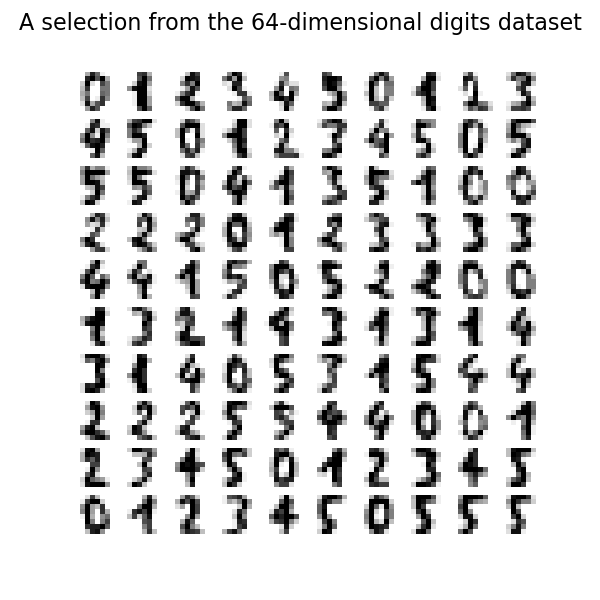
\includegraphics[width=.4\textwidth, trim=0 0 0 30, clip]{uci.png}
\end{frame}

\end{document}

